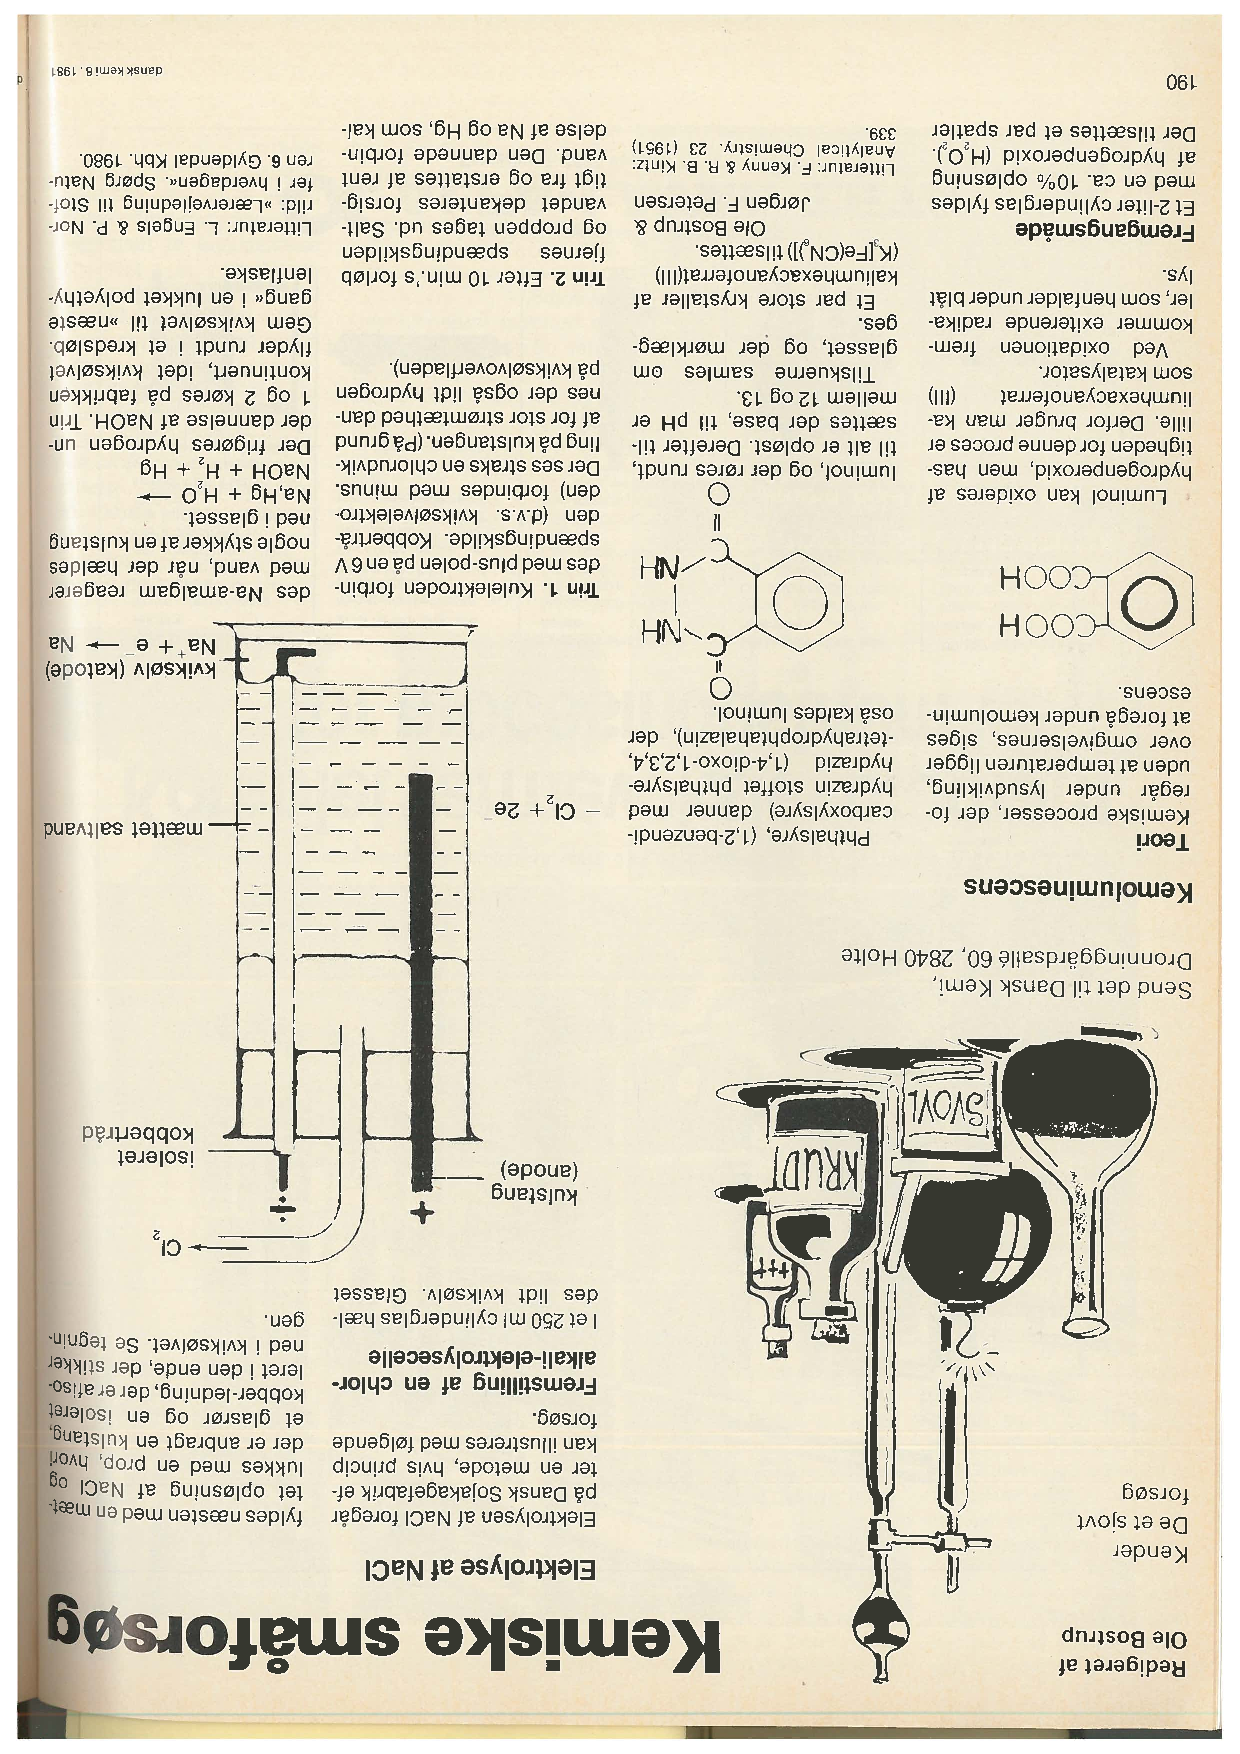
\includepdf[pages=-]{pdfs/1981-62-8-190.pdf}

\emne{Elektrolyse af NaCl}
\danskkemi{1981-62-8 190}
\forfatter{}

Elektrolysen af NaCl foregår på Dansk Sojakagefabrik efter en metode, hvis
princip kan illustreres med følgende forsøg.
\deloverskrift{Fremstilling af en chlor-alkali-elektrolysecelle.}
I et 250 ml cylinderglas hældes lidt kviksølv. Glasset fyldes næsten med en
mættet opløsning af NaCl og lukkes med en prop, hvori der er anbragt en
kulstang, et glasrør og en isoleret kobber-ledning, der er afisoleret.
